\documentclass[simplex.tex]{subfiles}
% NO NEED TO INPUT PREAMBLES HERE
% packages are inherited; you can compile this on its own
\providecommand{\mb}[1]{\boldsymbol{#1}}
\providecommand{\mv}[1]{\vec{#1}}
\providecommand{\ve}[1]{\boldsymbol{#1}}
\newcommand{\bpsi}{\ve{\psi}}
\newcommand{\bv}{\mb{v}}
\newcommand{\bx}{\mb{x}}

\onlyinsubfile{
\title{NeuroData SIMPLEX Report: Subfile}
}

\begin{document}
\onlyinsubfile{
\maketitle
\thispagestyle{empty}

The following report documents the progress made by the labs of Randal~Burns and Joshua~T.~Vogelstein at Johns Hopkins University towards goals set by the DARPA SIMPLEX grant.

%%%% Table of Contents
\tableofcontents

%%%% Publications
\bibliographystyle{IEEEtran}
\begin{spacing}{0.5}
\section*{Publications, Presentations, and Talks}
%\vspace{-20pt}
\nocite{*}
{\footnotesize	\bibliography{simplex}}
\end{spacing}
%%%% End Publications
}

\subsection{Discriminability}

We develop a measure of discriminability (or reliability).  It
is intuitive to understand and easy to implement.
Discriminability is defined to be the probability of within
subject distances being smaller than the cross subject
distances. If we let $x_{i,t}$ denote the t$^{\text{th}}$ trial of subject 
$i$ and $\Delta(,)$ be the metric, the (population) discriminability $D$
is: $D= P (\Delta(x_{i,t} , x_{i,t’}) \leq  \Delta(x_{i,t} , x_{i’,t’’}))$.
We want to search for the optimal processing pipeline which has the
maximal discriminability. 

During the last month, we have been trying to finalize the paper. Specifically, we formalize three algorithms and write the pseudocode for the algorithms. The three algorithms are computing sample discriminability from test and retest data set \ref{alg:dhat}, testing whether the data is better than random \ref{alg:ost}, and testing whether one processing pipeline is better than another \ref{alg:tst}. The pseudocode is provided below. For the R code and functions, please see \href{http://github.com/neurodata/discriminability}{neurodata/discriminability}.

Furthermore, we carry out the Algorithm \ref{alg:tst} on 13 fMRI data sets. Previously, we process 13 fMRI data sets with 64 pipelines, and show some pipelines yields data
sets with high sample discriminability. However, we do not have a valid test to compare different pipelines other than rank them by mean discriminability. We use the algorithm \ref{alg:tst} to carry out a two sample test to compare different pipelines for each data set. Specifically, all pipelines are compared to pipeline CFXSG. Then, a single p-values is calculated by applying Fisher's method to combine p-values from 13 sets. We group the pipelines by p-values and within each group the pipelines are ordered by mean discriminability. The result of rank graphs is shown in Figure \ref{fig:pipes}. The result of raw graphs can also be found \href{http://github.com/neurodata/discriminability}{here}. The new two sample test provide a better ordering of pipelines compared to the previous ordering by Wilcoxon signed-rank test. 

\begin{figure}[h!]
	\begin{cframed}
		\centering
		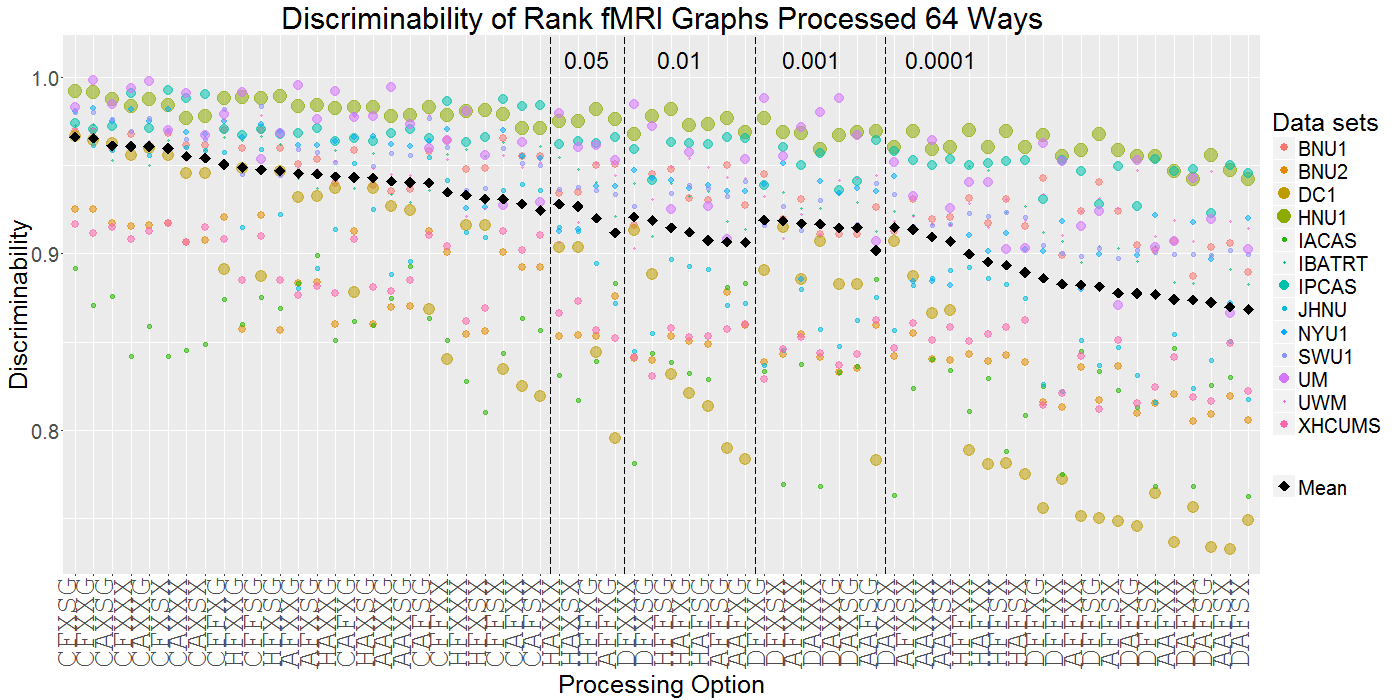
\includegraphics[width=\textwidth]{../../figs/fmri_rank_pv_v2.png}
		\caption{
			{\bf Discriminability of rank fmri graphs from 13 data sets processed 64 ways.}  Discriminability of BNU1, BNU2, DC1, HNU1, IACAS, IBATRT, IPCAS, JHNU, NYU1, SWU1, UM, UWM and XHCUMS pre-processed by 64 pipelines are shown in the plot. Color of each dot indicates data set and size indicates the number of measurements in data set. The black square indicates the weighted mean discriminability across 13 data sets.  For each data set, all pipelines are compared to the pipeline CFXSG using the two sample test, and a single p-value is calculated by Fisher's method. The pipelines are grouped by p-values. The number at the top indicates the range of the p-values. Within each group, the pipelines are ordered by the mean discriminability. CFXSG pipeline has the best mean discriminability across data sets.}
		\label{fig:pipes}
	\end{cframed}
\end{figure}

\subsubsection*{Discriminability Algorithms}
\begin{algorithm}               
	\caption{Compute discriminability estimate $\hat{D}$.  }   
	\label{alg:dhat}                       
	\begin{algorithmic}                    
		\Require Test-retest samples $\{\bx_{i,t}\}$.
		\Ensure Sample discriminability $\hat{D}$. 
		\Function{ComputeDiscriminability}{}
		\For{$i,t,i',t'$} \Comment{compute pairwise distances}
		\State $PD[i,t,i',t'] = \delta(\bx_{i,t},\bx_{i',t'})$
		\EndFor
		\State Dsum = 0;
		\State Count = 0;
		\For{$i = 1,...,n$} 
		\For{$t = 1,...,s$}
		\State $d =$ across subject distances to $\bx_{i,t}$
		\For{$t' = 1,...,s$ and $t' \neq t$}
		\State $\hat{D}_{i,t,t'} =\sum_j {\bf I}\{PD[i,t,i,t'] < d[j]\}/Length(d)$ \Comment{compare within and across distances}
		\State $Dsum = Dsum + \hat{D}_{i,t,t'}$
		\State $Count = Count + 1$
		\EndFor	
		\EndFor
		\EndFor
		\State $\hat{D} = Dsum / Count$ \Comment{Sample Discrminability}
		\EndFunction
	\end{algorithmic}
\end{algorithm}

\begin{algorithm}               
	\caption{The function returns a p-value for testing the null hypothesis that $D = 0.5$.  }   
	\label{alg:ost}                       
	\begin{algorithmic}                    
		\Require Test-retest samples $\{\bx_{i,t}\}$, the number of permutations $np$.
		\Ensure The p-value $p \in [0,1]$ for testing the hypothesis that $D = 0.5$. 
		\Function{OneSampleTest}{}
		\State $\hat{D}= ComputeDiscriminability(\{\bx_{i,t}\})$ \Comment{compute true sample discriminability}
		\For{$j = 1,...,np$} 
		\State $\{\bx^{(j)}_{i,t}\} = Permute(\{\bx_{i,t}\})$ \Comment{permute the subject labels}
		\State $d[j] = ComputeDiscriminability(\{\bx^{(j)}_{i,t}\})$ \Comment{compute discriminability of permuted samples}
		\EndFor
		\State $p = \sum_j {\bf I}\{\hat{D} < d[j]\} / np$ \Comment{compute p-value}
		\EndFunction
	\end{algorithmic}
\end{algorithm}

\begin{algorithm}               
	\caption{The function returns a p-value for testing the null hypothesis that $D(\bpsi_1)=D(\bpsi_2)$.  }   
	\label{alg:tst}                       
	\begin{algorithmic}                    
		\Require Raw data $\{f_\phi(\bv_i)\}$ , pipeline $\bpsi_1$, pipeline $\bpsi_2$, the number of bootstrapped samples $nb$.
		\Ensure The p-value $p \in [0,1]$ for testing the hypothesis that $D(\bpsi_1)=D(\bpsi_2)$. 
		\Function{TwoSampleTest}{}
		\State $\{^1\bx_{i,t}\}= g_{\bpsi_1}(\{f_\phi(\bv_i)\})$ 
		\State $\{^2\bx_{i,t}\}= g_{\bpsi_1}(\{f_\phi(\bv_i)\})$ \Comment{process the raw data with two pipelines}
		\State $\hat{D}(\bpsi_1)=ComputeDiscriminability(\{^1\bx_{i,t}\})$
		\State $\hat{D}(\bpsi_2)=ComputeDiscriminability(\{^1\bx_{i,t}\})$ \Comment{compute sample discriminability estimates}
		\For{$j = 1,...,nb$} 
		\For{$i = 1,...,n$} 
		\State $i_1, i_2 = Sample(n)$ \Comment{randomly select two subjects}
		\State $\lambda = SampleUniform$ 
		\For{t = 1,...,s}  
		\State $^1\bx^{(j)}_{i,t} =  ^1\bx_{i_1,t} \lambda +   ^1\bx_{i_2,t}(1-\lambda)$ \Comment{Linearly combine two observations}
		\EndFor
		\EndFor
		\State $\hat{D}^{(j)}(\bpsi_1)=ComputeDiscriminability(\{^1\bx^{(j)}_{i,t}\})$
		\State $\hat{D}^{(j)}(\bpsi_2)=ComputeDiscriminability(\{^2\bx^{(j)}_{i,t}\})$
		\EndFor
		\State $ind = 0$
		\For{$j = 1,...,nb$} \Comment{generate the null distribution}
		\For{$j' = i+1,...,nb$}
		\State $d[ind] =  \hat{D}^{(j)}(\bpsi_1)-\hat{D}^{(j')}(\bpsi_1)$ 
		\State $ind = ind + 1$
		\State $d[ind] =  \hat{D}^{(j)}(\bpsi_2)-\hat{D}^{(j')}(\bpsi_2)$
		\State $ind = ind + 1$
		\EndFor
		\EndFor
		\State $p = \sum_j {\bf I}\{\hat{D}(\bpsi_1)-\hat{D}(\bpsi_2) < d[j]\} / Length(d)$ \Comment{compute p-value}
		\EndFunction
	\end{algorithmic}
\end{algorithm}


  







\end{document}
